\chapter{Thực nghiệm}
\label{chap:Experiment}

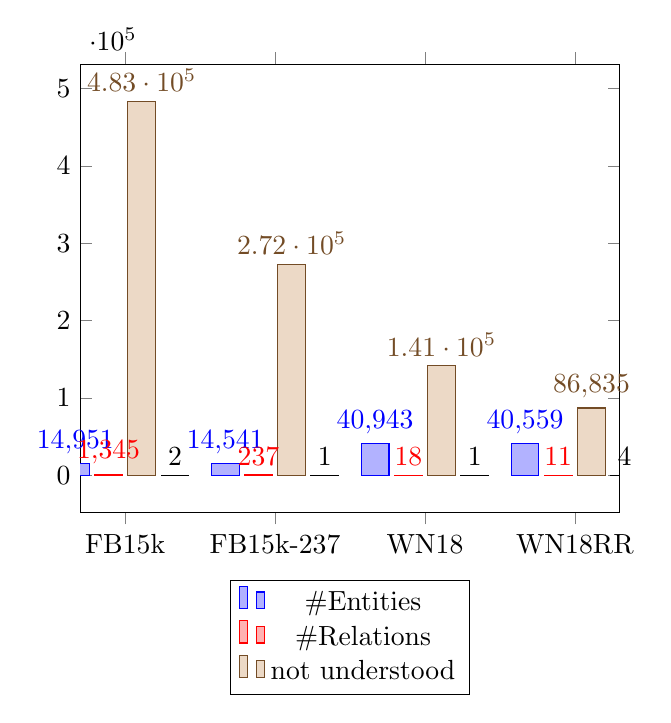
\begin{tikzpicture}
	\begin{axis}[
		ybar,
		legend style={at={(0.5,-0.15)}, anchor=north},
		symbolic x coords={FB15k,FB15k-237,WN18, WN18RR},
		xtick=data,
		nodes near coords,
		nodes near coords align={vertical},
		]
		\addplot coordinates {(FB15k, 14951) (FB15k-237,14541) (WN18,40943) (WN18RR,40559)};
		\addplot coordinates {(FB15k,1345) (FB15k-237,237) (WN18,18) (WN18RR,11)};
		\addplot coordinates {(FB15k,483142) (FB15k-237,272115) (WN18,141442) (WN18RR, 86835)};
		\addplot coordinates {(FB15k,2) (FB15k-237,1) (WN18,1) (WN18RR,4)};
		\legend{\#Entities,\#Relations,not understood}
	\end{axis}
\end{tikzpicture}

Trong phần này chúng tôi mô tả lại các bộ dữ liệu mà chúng tôi dùng để thực nghiệm đánh giá phương pháp của chúng tôi cùng với so sánh với các kết quả khác của các công trình nổi bật khác được báo cáo trong \hyperref[tab:tab1]{bảng 2.1}. Ngoài ra chúng tôi cũng cố gắng đánh giá hai đề xuất của chúng tôi trong việc thêm một lượng tri thức mới vào đồ thị bằng cách chúng tôi xem tập test là một lượng tri thức mới cần thêm vào và dùng tập vadidation để đánh giá lại phương pháp của chúng tôi. Kết quả chi tiết được báo cáo ở \hyperref[tab:tab1]{bảng 2.2}

\begin{table}[htbp]
	\begin{center}
		\resizebox{\textwidth}{!}{%
			\begin{tabular}{lllllll}
				\hline
				&          &           & \multicolumn{4}{l}{\# Edges}    \\ \cline{4-7}
				
				Dataset   & Entities & Relations & Training & Validation & Test   & Total   \\ \hline
				FB15k     & 14,951   & 1,345     & 483,142  & 50,000     & 59,071 & 592,213 \\
				FB15k-237 & 14,541   & 237       & 272,115  & 17,535     & 20,466 & 310,116 \\
				WN18      & 40,943   & 18        & 141,442  & 5,000      & 5,000  & 151,442 \\
				WN18RR    & 40,559   & 11        & 86,835   & 3034       & 3134   & 93,003 \\
				\hline
			\end{tabular}
		}
		\caption{Thông tin các tập dữ liệu}
		\label{tab:dataset}
	\end{center}
\end{table}


\section{Các tập dữ liệu huấn luyện}
\label{sec:DataTraining}

Trong thí nghiệm của chúng tôi, chúng tôi thực hiện trên bốn tập dữ liệu phổ biến là FB15k, FB15-237, WN18 và WN18RR.Các bộ dữ liệu này là tập hợp các bộ ba (triple) \(\langle head, relation, tail \rangle\) biểu thị cho thực thể đầu có một mối quan hệ với thực thể cuối.

\subsection{Bộ dữ liệu FB15k}

Bộ dữ liệu này được tạo bởi nhóm nghiên cứu A. Bordes, N. Usunier, A. Garcia-Duran, J. Weston, and O. Yakhnenko \cite{bordes2013translating} bằng cách trích xuất từ bộ dữ liệu Wikilinks database \footnote{https://code.google.com/archive/p/wiki-links/}.Wikilinks database thu thập các siêu liên kết(hyperlinks) đến Wikipedia gồm 40 triệu lượt đề cập trên 3 triệu thực thể, họ trích xuất tất cả các dữ kiện liên quan đến một thực thể nhất định có hơn 100 lần được đề cập đến bởi các tài liệu khác cùng với tất cả các dữ kiện liên quan đến thực thể đó (bao gồm cả những thực thể con được nhắc đến trong tài liệu Wikipedia đó), ngoại trừ những thonng tin như: ngày tháng, danh từ riêng, v.v ... Họ cũng chuyển đổi các đỉnh có bậc \(n\) được biểu diễn thành các nhóm các cạnh nhị phân tức là liệt kê các cạnh và quan hệ của mọi đỉnh. Tập dữ liệu được chia ngẫu nhiên thành 3 tập: tập training với 1345 relations, 14834 head entities và 14903 tail entities, tập test gồm 916 relations, 11886 head entities, và 11285 tail entities, tập validation gồm 961 relations, 12297 head entities, và 11825 tail entities.

\subsection{Bộ dữ liệu FB15k-237}

Bộ dữ liệu này là một tập hợp con của FB15k được xây dựng bởi Toutanova và Chen \cite{toutanova2015observed} lấy cảm hứng từ quan sát rằng FB15k bao gồm dữ liệu thử nghiệm được các mô hình nhìn thấy tại thời điểm đào tạo (test leekage). Trong FB15k, vấn đề này là do sự hiện diện của các quan hệ gần giống nhau hoặc nghịch đảo của nhau.FB15k-237 được xây dựng để trở thành một tập dữ liệu thách thức hơn: các tác giả đã chọn các dữ kiện liên quan đến 401 quan hệ xuất hiện nhiều nhất và loại bỏ tất cả các quan hệ tương đương hoặc nghịch đảo. Họ cũng đảm bảo rằng không có thực thể nào được kết nối trong tập huấn luyện cũng được liên kết trực tiếp trong tập test và validation.Tập training gồm 237 relations, 13781 head entities, và 13379 tail entities, tập test gồm 223 relations, 7652 head entities, và 5804 tail entities, tập vadition gồm 224 relations, 8171 head entities, and 6376 tail entities.

\subsection{Bộ dữ liệu WN18}

Bộ dữ liệu này được giới thiệu bởi các tác giả của TransE \cite{bordes2013translating}, được trích xuất từ WordNet\footnote{https://wordnet.princeton.edu/}, một bản thể học ngôn ngữ KG có nghĩa là cung cấp một từ điển/từ đồng nghĩa để hỗ trợ NLP và phân tích văn bản tự động. Trong WordNet, các thực thể tương ứng với các tập hợp (\textit{word senses}) và các quan hệ đại diện cho các kết nối từ vựng của chúng (ví dụ: “hypernym”). Để xây dựng WN18, các tác giả đã sử dụng WordNet làm điểm bắt đầu và sau đó lặp đi lặp lại lọc ra các thực thể và mối quan hệ với quá ít lần được đề cập. Tập dữ liệu được chia ngẫu nhiên thành 3 tập: tập training với 18 relations, 40504 head entities, và 40551 tail entities, tập test gồm 18 relations, 4262 head entities, and 4338 tail entities, tập vadiation gồm 18 relations, 4349 head entities, and 4263 tail entities.

\subsection{Bộ dữ liệu WN18RR}

Bộ dữ liệu này là một tập hợp con của WN18 được xây dựng bởi DeŠmers et al.\cite{dettmers2017convolutional}, cũng là người giải quyết vấn đề rò rỉ thử nghiệm (test leakage)trong WN18. Để giải quyết vấn đề đó, họ xây dựng tập dữ liệu WN18RR thách thức hơn nhiều bằng cách áp dụng một phương pháp tương tự được sử dụng cho FB15k-237 \cite{toutanova2015observed}. Training gồm 11 relations, 39610 head entities, và 31881 tail entities, tập test gồm 11 relations, 2958 head entities, và 2619 tail entities, tập vadition gồm 11 relations, 2851 head entities, and 2575 tail entities.

\section{Các độ đo}
Trong phần này chúng tôi mô tả lại các phương pháp đánh giá (độ do), môi trường thực hiện cũng như các tập dữ liệu mà chúng tôi sử dụng để dánh giá phương pháp của mình. Các phương pháp đánh giá (độ do) này cũng phổ biến nó được đánh giá cho hầu hết các mô hình dự đoán liên kết trên đồ thị. Chúng tôi tiến hành so sánh với bốn phương pháp nổi bật khác được báo cáo trong \cite{rossi2020knowledge}.

\subsubsection{Độ đo Hit@K (H@K)}

Đó là tỷ lệ các dự đoán đúng mà rank nhỏ hơn hoặc bằng ngưỡng \(K\):
\[H@K = \frac{\mid {q ~\in ~Q~: rank(q) \leq K} \mid}{\mid Q \mid}\]

\subsubsection{Mean Rank (MR)}

Đây là giá trị trung bình của rank thu được cho một dự đoán chính xác. Càng nhỏ thì mô hình càng chính xác:
\[MR = \frac{1}{\mid Q \mid} \sum_{q ~\in~ Q} rank(q) \]
Trong đó \(\mid Q \mid\) là độ lớn của tập hợp các câu hỏi bằng độ lớn của tập test hoặc vadidation. Khi dự đoán chúng tôi dự đoán cả head và tail cho một dòng tương ứng trong tập dữ liệu thử nghiệm. Ví dụ chún tôi sẽ dự đoán \(\langle ?,~ relation,~ tail \rangle\) và \(\langle head,~ relation,~ ?\rangle\) cho 1 dòng tương ứng, \(q\) thể hiện cho câu hỏi chúng tôi dự đoán và \(rank(q)\) thể hiện cho kết quả đúng của câu hỏi đứng ở vị trí thứ mấy trong xếp hạng của chúng tôi sau đó lấy trung bình rank của các dự đoán head và tail. Rõ ràng độ đo này nằm giữa \([1, \mid \text{số lượng các entity} \mid]\) do có tối da \(n\) cạnh nối 1 đỉnh tới \(n-1\) đỉnh còn lại và thêm cạnh nối tới chính đỉnh nó(cạnh khuyên). Và độ đo này đễ bị ảnh hưởng bởi nhiễu vì có những quan hệ có những thực thể được xếp hạng gần cuối. Để giải quyết vấn đề này nhóm chúng tôi và các nhóm nghiên cứu khác sử dụng thêm độ đo Mean Reciprocal Rank (MMR)

\subsubsection{Mean Reciprocal Rank (MMR)}

Đây là xếp hạng đối ứng trung bình, là nghịch đảo của giá trị trung bình của rank thu được cho một dự đoán chính xác ở trên. Và càng lớn thì mô hình càng chính xác. Do độ đo này lấy nghịch đảo của các rank nên tránh dược vấn đề nhiễu của độ đo MR ở trên.
\[MRR =\frac{1}{\mid Q \mid} \sum_{q~ \in ~Q} \frac{1}{rank(q)}\]

\section{Phương pháp huấn luyện}

\subsection{Huấn luyện trên mô hình AnyBURL}


\subsection{Huấn luyện trên mô hình GCAT}

Chúng tôi sử dụng Google Colab Pro để huấn luyện tập dữ liệu
........

\section{Kết quả thực nghiệm}
\label{sec:Experiment}

Như đã nói trước đây với mô hình dựa trên luật của chúng tôi hoàn toàn có thể thực hiện trên một laptop với cấu hình thông thường. Trong thí nghiệm của chúng tôi cấu hình máy để thực thi như sau: T480, core i5 8th Gen, ram 16Gb, 4 core 8 thread. Mã nguồn thực thi được viết bằng ngôn ngữ Python phiên bản 3.6 và dùng các hàm hỗ trợ có sẵn trong Python với không một thư viện bên thứ ba nào. Thí nghiệm được thực hiện với bốn tập dữ liệu phổ biến là FB15k, FB15-237, WN18 và WN18RR. Thông tin chi tiết các bộ dữ liệu này được mô tả ở phần \hyperref[datasets]{các tập dữ liệu huấn luyện}.

Như mô tả ở phần \hyperref[algorithm2]{thuật toán AnyBURL} thuật toán này sẽ học các luật được sinh ra trong một khoảng thời gian nhất định do người dùng cấu hình. Ở đây chúng tôi chọn cấu hình thời gian là 1000 giây tương đương khoảng 17 phút đào tạo, với độ bão hòa(SAT) \(0.85\), độ tin cậy Q \(0.05\), kích thước mẫu S (\(\frac{1}{10}~ \text{tập huấn luyện}\)). Với cấu hình như vậy mô hình phiên bản Python của chúng tối cho kết quả tương đương với phiên bản Java nhóm tác giả Meilicke, Christian et al. \cite{burl} với cấu hình tương tự nhưng thời gian training là 100 giây. Sự khác biệt về thời gian học tập ở đây chủ yếu là do hiệu năng của hai ngôn ngữ Python và Java. Ở đây chúng tôi chọn ngôn ngữ Python vì nó được dùng làm ngôn ngữ chính cho nhiều mô hình trí tuệ nhân tạo gần đây, và cũng thuận tiện cho chúng tôi khi so sánh hiệu năng cũng như đánh giá với các phương pháp học sâu khác đa số được viết bằng Python.

\hyperref[tab:tab1]{Bảng 4.1}, và \hyperref[tab:tab2]{bảng 4.2} bên dưới mô tả các kết quả thực nghiệm của chúng tôi với các độ đo \(H@K\) cùng với các kết quả thực nghiệm của các phương pháp khác được đề cập trong khảo  sát \cite{rossi2020knowledge}

\begin{table}[ht]
	\begin{center}
		\resizebox{\textwidth}{!}{%
			\begin{tabular}{l|l|l|l|l|l|l|l|l|}
				\cline{2-9}
				& \multicolumn{4}{c|}{\textbf{FB15k}}                   & \multicolumn{4}{c|}{\textbf{FB15k-237}}                   \\ \cline{2-9} 
				& \textbf{H@1} & \textbf{H@10} & \textbf{MR} & \textbf{MRR} & \textbf{H@1} & \textbf{H@10} & \textbf{MR} & \textbf{MRR} \\ \hline
				\multicolumn{1}{|l|}{ComplEx} & 81.56        & 90.53         & 34          & 0.848        & 25.72        & 52.97         & 202        & 0.349        \\ \hline
				\multicolumn{1}{|l|}{TuckER}  & 72.89        & 88.88         & 39          & 0.788        & 25.90        & 53.61         & 162         & 0.352        \\ \hline
				\multicolumn{1}{|l|}{TransE}  & 49.36        & 84.73         & 45          & 0.628        & 21.72        & 49.65         & 209         & 0.31        \\ \hline
				\multicolumn{1}{|l|}{RoteE}   & 73.93        & 88.10         & 42          & 0.791        & 23.83        & 53.06         & 178         & 0.336        \\ \hline
				\multicolumn{1}{|l|}{ConvKB}  & 59.46        & 84.94         & 51         & 0.688        & 21.90        & 47.62         & 281         &0.305        \\ \hline
				\multicolumn{1}{|l|}{\textbf{KBGAT}}     &  70.08            &     91.64    &  38    &   0.784    & 36.06     &    58.32   &  211  &    0.4353  \\ \hline
				\multicolumn{1}{|l|}{\textbf{AnyBURL}}    & \textbf{79.13}        & \textbf{82.30}         & \textbf{285}         & \textbf{0.824}        & \textbf{20.85}        & \textbf{42.40}         & \textbf{490}         & \textbf{0.311}        \\ \hline
			\end{tabular}
		}
		\caption{Kết quả phương pháp đề xuất trên FB15k, FB15k-237}
		\label{tab:tab1}%
	\end{center}
\end{table}

\begin{table}[ht]
	\begin{center}
		\resizebox{\textwidth}{!}{%
			\begin{tabular}{l|l|l|l|l|l|l|l|l|}
				\cline{2-9}
				& \multicolumn{4}{c|}{\textbf{WN18}}                              & \multicolumn{4}{c|}{\textbf{WN18RR}}                            \\ \cline{2-9} 
				& \textbf{H@1}   & \textbf{H@10}  & \textbf{MR}  & \textbf{MRR}   & \textbf{H@1}   & \textbf{H@10}  & \textbf{MR}  & \textbf{MRR}   \\ \hline
				\multicolumn{1}{|l|}{ComplEx} & 94.53          & 95.50          & 3623         & 0.349          & 42.55          & 52.12          & 4909         & 0.458          \\ \hline
				\multicolumn{1}{|l|}{TuckER}  & 94.64          & 95.80          & 510          & 0.951          & 42.95          & 51.40          & 6239         & 0.459          \\ \hline
				\multicolumn{1}{|l|}{TransE}  & 40.56          & 94.87          & 279          & 0.646          & 2.79           & 94.87          & 279          & 0.646          \\ \hline
				\multicolumn{1}{|l|}{RoteE}   & 94.30          & 96.02          & 274          & 0.949          & 42.60          & 57.35          & 3318         & 0.475          \\ \hline
				\multicolumn{1}{|l|}{ConvKB}  & 93.89          & 95.68          & 413          & 0.945          & 38.99          & 50.75          & 4944         & 0.427          \\ \hline
				\multicolumn{1}{|l|}{\textbf{KBGAT}}     &                &        &        &                &       35.12         &        57.01         &      1974       &  0.4301           \\ \hline
				\multicolumn{1}{|l|}{\textbf{AnyBURL}}    & \textbf{93.96} & \textbf{95.07} & \textbf{230} & \textbf{0.955} & \textbf{44.22} & \textbf{54.40} & \textbf{490} & \textbf{0.490} \\ \hline
			\end{tabular}
		}
		\caption{Kết quả phương pháp của chúng tôi trên WN18, WN18RR}
		\label{tab:tab2}%
	\end{center}
\end{table}

Bảng \hyperref[tab:tab3]{4.3} bên dưới mô tả các kết quả thực nghiệm của chúng tôi với hai chiến lược thêm tri thức mới vào đồ thị. Chúng tôi đánh giá trên tổng số luật được sinh ra, và số luật có độ tin cậy \(>= 50\%\) và \(>= 80\%\).

\begin{table}[ht]
	\begin{center}
		\begin{tabular}{ll|l|l|}
			\cline{3-4}
			& & \textbf{online-to-offline} & \textbf{online-to-online} \\ \hline
			\multicolumn{1}{|c|}{\multirow{3}{*}{\textbf{FB15k}}}     & num rule        & 1011                       & 1367                      \\ \cline{2-4} 
			\multicolumn{1}{|c|}{}& confidence 50\% & 416 (41,14\%)              & 1185 (86,69\%)            \\ \cline{2-4} 
			\multicolumn{1}{|c|}{}& confidence 80\% & 284 (28, 09\%)             & 481 (35,18\%)             \\ \hline
			\multicolumn{1}{|l|}{\multirow{3}{*}{\textbf{FB15k-237}}} & num rule        & 1120                       & 756                       \\ \cline{2-4} 
			\multicolumn{1}{|l|}{}& confidence 50\% & 244 (21,79\%)              & 660 (87,30\%)             \\ \cline{2-4} 
			\multicolumn{1}{|l|}{}& confidence 80\% & 95 (8,48\%)                & 162 (21,43\%)             \\ \hline
			\multicolumn{1}{|l|}{\multirow{3}{*}{\textbf{WN18}}}      & num rule        & 533                        & 260                       \\ \cline{2-4} 
			\multicolumn{1}{|l|}{}& confidence 50\% & 270 (38, 46 \%)            & 252 (96,92\%)             \\ \cline{2-4} 
			\multicolumn{1}{|l|}{}& confidence 80\% & 240 (34,19\%)              & 225 (86,54\%)             \\ \hline
			\multicolumn{1}{|l|}{\multirow{3}{*}{\textbf{WN18RR}}}    & num rule        & 439                        & 106                       \\ \cline{2-4} 
			\multicolumn{1}{|l|}{}& confidence 50\% & 110 (25,05\%)              & 102 (96,22\%)             \\ \cline{2-4} 
			\multicolumn{1}{|l|}{}& confidence 80\% & 83 (18,91\%)               & 85 (81,19\%)              \\ \hline
		\end{tabular}
		\caption{Kết quả hai chiến lược thêm tri thức mới}
		\label{tab:tab3}%
	\end{center}
\end{table}